\documentclass{article}
\usepackage{amsmath}
\usepackage{amssymb}
\usepackage{graphicx}
\usepackage{hyperref}
\usepackage[version=4]{mhchem}


\begin{document}
\section*{Problem}
(AMC) In \(\triangle A B C, M\) is the midpoint of side \(B C, A N\) bisects \(\angle B A C\), \(B N \perp A N\) and \(\theta\) is the measure of \(\angle B A C\). If sides \(A B\) and \(A C\) have lengths 14 and 19 , respectively, then length \(M N\) equals\\
(A) 2\\
(B) \(\frac{5}{2}\)\\
(C) \(\frac{5}{2}-\sin \theta\)\\
(D) \(\frac{5}{2}-\frac{1}{2}\) \(\sin \theta\)\\
(E) \(\frac{5}{2}-\frac{1}{2} \sin \left(\frac{\theta}{2}\right)\)\\
\centering
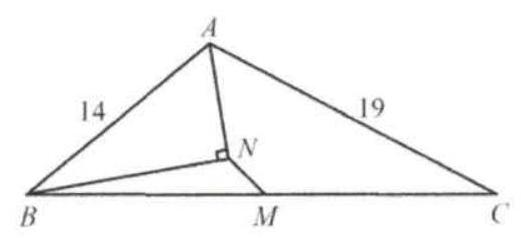
\includegraphics[width=\textwidth]{images/064.jpg}

\section*{Solution}
(B).
In the adjoining figure, \(B N\) is extended past \(N\) and meets \(A C\) at \(E\). Triangle \(B N A\) is congruent to \(\triangle E N A\), since \(\angle B A N=\angle E A N, A N=\) \(A N\) and \(\angle A N B=\angle A N E=90^{\circ}\).

Therefore \(N\) is the midpoint of \(B E\), and \(A B=A E=\) 14. Thus \(E C=5\). Since \(M N\) is the line joining the midpoints of sides \(B C\) and \(B E\) of \(\triangle C B E\), its length\\
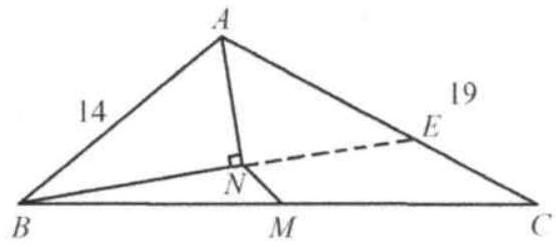
\includegraphics[width=\textwidth]{images/067(2).jpg} is \(\frac{1}{2} E C=\frac{5}{2}\).

\end{document}
